Un componente importante para la implementación de la arquitectura planteada es la memoria cache compartida, la cual evitará accesos innecesarios a los backends, obteniendo mejores tiempos de respuesta.  Según la RFC 7234\footnote{Este documento define las caches \gls{proto:http} y las cabeceras de control de cache permitidas en la versión \texttt{1.1} de ese protocolo\\\url{https://tools.ietf.org/html/rfc7234}}, una memoria cache almacena respuestas en pos de reducir el tiempo de respuesta y el consumo del ancho de banda. Asimismo, una memoria cache compartida es una cache que almacena respuestas para ser usadas por más de un cliente.

En este apartado nos centraremos en los tipos de memorias compartidas \eng{proxy server} y \eng{reverse proxy server}.  Un \eng{proxy server}, también conocido como \eng{forward proxy server}, actúa como un proxy para los dispositivos que se conectan a él.  Una implementación típica puede ser un \eng{forward proxy} que provee acceso a internet a N clientes.
En cambio, un \eng{reverse proxy server} es un servidor proxy que recupera recursos desde uno o mas servidores.  Estos recursos se devuelven al cliente como si se hubieran originado desde el propio servidor, es decir, actúa como intermediario entre los clientes y servidores.  Los \eng{reverse proxys} se implementan en las proximidades de los \eng{web servers}, a veces realizan tareas como balanceo de carga, autenticación, o \eng{caching}.

\begin{figure}[H]
  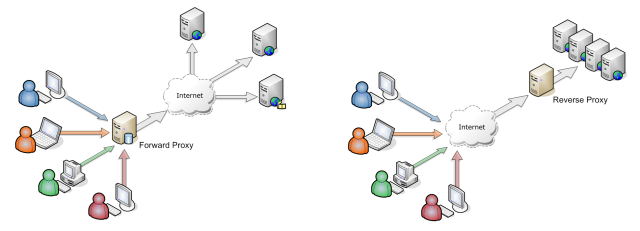
\includegraphics[width=\linewidth]{src/images/03-capitulo-3/tecnologias/squid/forward-reverse-proxy.png}
  \caption{Forward proxy y reverse proxy}
  \label{fig:varnish}
\end{figure}
